\subsubsection{Flash Proxy}
Flash Proxy \cite{FlashProxy} is another client add-on tool that helps in avoiding censorship. It creates a “short-life” proxy and it can connect to created proxies around the globe, so when users try to join Tor, they can connect to this proxy (since it is difficult to be blocked) and then to Tor.

\begin{figure}[!h]
 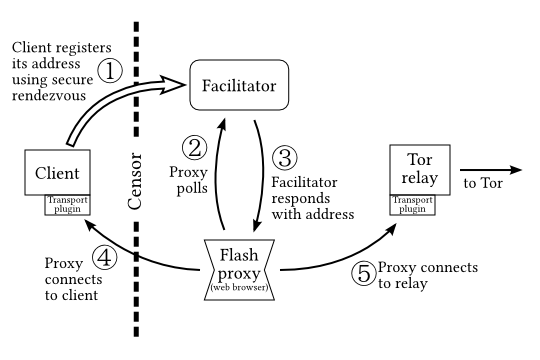
\includegraphics[width=16cm]{flashProxy}
 \caption{How Flash Proxy works}
\end{figure}